\documentclass[border=4pt]{standalone}
\usepackage{pgfplots}
\pgfplotsset{compat=1.18}

\begin{document}
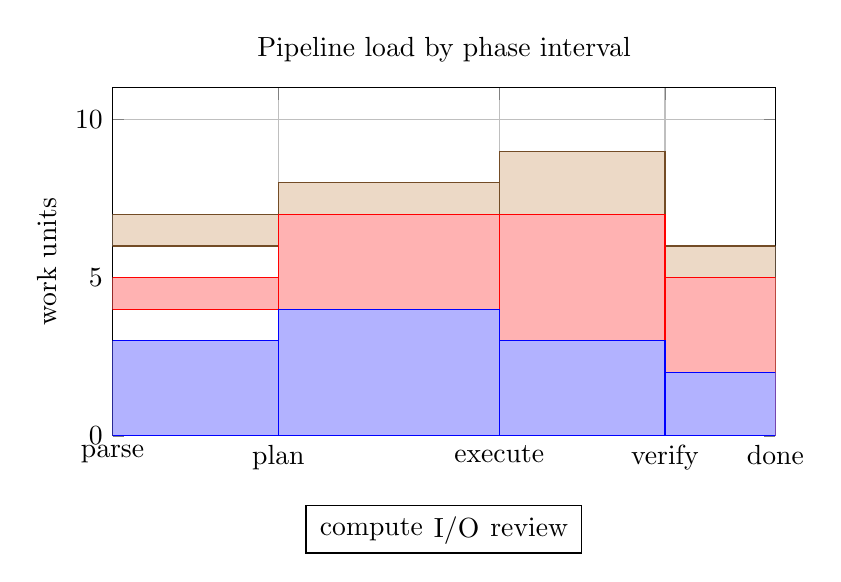
\begin{tikzpicture}
  \begin{axis}[
    ybar interval stacked,
    width=10cm,
    height=6cm,
    xmin=0,
    xmax=6,
    ymin=0,
    ymax=11,
    xtick={0,1.5,3.5,5,6},
    xticklabels={parse,plan,execute,verify,done},
    ylabel={work units},
    title={Pipeline load by phase interval},
    grid=major,
    legend style={at={(0.5,-0.2)},anchor=north,legend columns=-1}
  ]
    \addplot coordinates {(0,3) (1.5,4) (3.5,3) (5,2) (6,0)};
    \addplot coordinates {(0,2) (1.5,3) (3.5,4) (5,3) (6,0)};
    \addplot coordinates {(0,1) (1.5,1) (3.5,2) (5,1) (6,0)};
    \legend{compute,I/O,review}
  \end{axis}
\end{tikzpicture}
\end{document}
